\documentclass[letterpaper,12pt]{article}

\RequirePackage{GE05}
% this inputs graphicx, too
\RequirePackage{comment}
\RequirePackage[hypertex]{hyperref}
%\hypersetup{dvips}
%\hypersetup{backref,colorlinks=false,urlcolor=cyan,linkcolor=blue}
%\hypersetup{pdfpagemode=None,pdfstartview=FitH}

% Example counter and macro
\newcounter{exhibit}
\setcounter{exhibit}{1}
\newcommand{\exhibit}[1]{%
    \noindent{\bf Exhibit \arabic{exhibit}. #1.}%
    \addtocounter{exhibit}{1}
    }

\def\ClassName{The Global Economy}
\def\Category{Mini-Case}
\def\HeadName{Is China's Currency ``Undervalued''?}

\begin{document}
\parindent = 0.0in
\parskip = 0.7\bigskipamount
\thispagestyle{empty}%
\Head

\centerline{\large \bf \HeadName}%
\centerline{Revised:  \today}

\bigskip 
China's currency gets a lot of attention in the United States and 
elsewhere, with some suggesting that China maintains a cheap 
currency to support its exports.  
Examples include:
% 
\begin{itemize}
\item Senator Charles Schumer of New York:
``It's time to put some muscle into our trade relationship with China. 
For too long, the Chinese government has been playing games with the value of its currency in order to get a competitive edge.''

\item Nobel laureate and political pundit Paul Krugman:  
``Here's how it works: Unlike the dollar, the euro or the yen, whose values fluctuate freely, China's currency is pegged by official policy at about 6.8 yuan to the dollar.  At this exchange rate, Chinese manufacturing has a large cost advantage over its rivals, leading to huge trade surpluses.
Under normal circumstances, the inflow of dollars from those surpluses would push up the value of China's currency, unless it was offset by private investors heading the other way.  And private investors are trying to get into China, not out of it. But China's government restricts capital inflows, even as it buys up dollars and parks them abroad, adding to a \$2 trillion-plus hoard of foreign exchange reserves.''  
\end{itemize}
%
All of us have seen similar comments from experts:  
that China's currency is undervalued as a result 
of government policies.  


Are they right?  
Has China has somehow arranged for 
the price of its currency to be too low?  
Is its currency undervalued?  Manipulated?  
Your mission is to decide, first, 
what undervalued means and, second, 
to make a persuasive case for or against 
undervaluation and 
active currency manipulation by the Chinese government.  


\subsubsection*{Valuing China's currency}

First some terminology:  
China's currency is the {\it renminbi\/} (or RMB) 
but units of currency are referred to as {\it yuan\/}. 
Thus you would exchange dollars for renminbi at the airport
but quote prices in yuan.

Exhibit 1 shows how the dollar-RMB exchange rate has changed over
the last 30 years.  
Since the late 1980s, periods in which the exchange rate was fixed 
(the flat segments) have been interspersed with periodic upward 
adjustments, some of them sudden and substantial, 
in which the RMB declined in value.  
Since 2005 the RMB has slowly appreciated, 
rising in value by 20\% between mid-2005 and early 2010.  
%We'll talk later about some of the policy changes that accompanied
%these movements.  

The depreciation of the early 1990s reflected, in large
part, Chinese inflation.  
Exhibit 2 shows the inflation rates, 
with inflation significantly higher in China from 1992-1998 
and only modestly different since then.  
Exhibit 3 compares the nominal exchange rate 
($s$ in the notation we've used in class)  
to the price ratio ($P/P^*$, with China as the domestic country).
Exhibit 4 puts these ingredients together as
a real exchange rate ($sP^*/P$):  
the ratio of Chinese prices to US prices, 
with both expressed in the same units.  
Although there has been some variation over time, 
the real exchange rate is not much different now than 
it was in 1990.  

With this evidence in hand, 
how would you go about
deciding whether a currency was valued appropriately?  
The conventional approach to that question is based on 
some version of purchasing power parity:
the theory that says exchange rates equate 
the purchasing power (the ``parity,'' some would say)
of currencies across countries.
If a product or collection of products sells for (say) \$100
in the US, it should sell for the same price in France, 
Japan, and even China once we convert their prices to dollars. 
Purchasing power parity applies this idea to consumer price indexes
such as those used in Exhibits 2-4.  

If this seems like a reasonable idea, 
there are a number of difficulties applying it in practice.  
Here's a list:   
%
\begin{enumerate}

\item Our PPP comparison is based on price indexes.
Since the scale of an index is arbitrary 
(index = 100 in 1990, for example), 
it's not a complete comparison of prices.
It would be nice to have a complete set of prices
that are comparable across countries, but we don't. 
When we look at prices of Big Macs, 
we see that they're substantially lower
in China (\$1.83 in China v. \$3.58 in the US in early 2010).  
Big Macs may not be typical, but when we try to expand 
on this idea  we run into:  

\item Chinese price data is notoriously bad.  
The OECD's {\it Economic Survey:  China\/} put it this way in 2005:
%
\begin{quote}
The OECD and other international organisations have collaborated
in the International Comparisons Project (ICP) to provide
estimates of purchasing power parities across countries.
To date, China has never fully participated.
It intends to participate in the near future, but then only for 11 urban areas
rather than nationwide.  
In the absence of ICP estimates, there have been a wide variety of 
alternative estimates.  
The variation in estimated parities is extreme.  
\end{quote}
%
Many experts think the data is passable for measuring inflation
inside China but inadequate for direct comparisons 
of prices across countries.  

\item Prices tend to be lower in poor countries generally. 
This is a fact, and provides some basis for lower prices in China.
Whether it's enough to account for apparent differences is up for debate.  

\end{enumerate} 

The result is a wide range of opinion 
on the appropriate value for the RMB.  
The ambiguity is reflected in public debate and official policy statements.  
This statement comes from the IMF Executive Board Article IV Consultation  
on July 22, 2009:  

%\href{http://www.imf.org/external/np/sec/pn/2009/pn0987.htm}{link}
\begin{quote}
[IMF] Directors welcomed the important progress made in the past few years in increasing the market's role in determining the exchange rate. ...
Some Directors nevertheless supported the view that the renminbi remains substantially undervalued. ... A number of other Directors pointed to the methodological difficulties of making exchange rate assessments.  These Directors generally considered that exchange rate appreciation would only play a supplementary role in supporting reforms to reorient the Chinese economy and should be pursued in a gradual manner, as and when conditions permit.
\end{quote} 

A VoxEU report edited by Simon Evenett 
summarized the evidence this way:  
``China's currency is undervalued by somewhere between 2.5\% and 27.5\%.''


\subsubsection*{The market for Chinese currency}

Another source of tension is the process by which the 
Chinese exchange rate is determined.
In the US, exchange rates are determined by market forces, 
but indirectly influenced by government policy, particularly
monetary policy.
In many developing countries, 
exchange rates are fixed and the central bank or treasury
intervenes routinely to maintain the price.  
``Convertibility'' may also be an issue:  
some currency transactions 
may be restricted or prohibited altogether.  


China not only intervenes in currency markets to control the 
exchange rate, 
it also places severe restrictions
on private transactions in currency markets.  
There has been steady progress in weakening these restrictions, 
but individuals and businesses operating in China face 
limitations on currency transactions that 
individuals and businesses in (say) the US do not.  
Many of these are enforced by the State Administration on 
Foreign Exchange (SAFE).  
The following summary is based on the 2009 Economist Intelligence Unit
{\it Country Finance\/} report.
%
\begin{itemize}
\item In December 1996, China removed restrictions on 
``convertibility for current account transactions.''
In common language, this means that foreign exchange transactions 
are permitted for importing, exporting, paying or receiving interest
on foreign loans, and so on.  
These transactions are permitted, but typically require approval.  
Prohibitions remain on many ``capital account'' transactions:  
purchases and sales of assets.  

\item International purchases and sales of assets remain restricted, 
whether Chinese transactions in foreign assets or 
foreign transactions in Chinese assets, 
and currency restrictions are layered on top.  
Direct investment in Chinese companies is permitted in some
sectors, and not in others.  
Approved investments can then be approved for the required currency
transactions.  
Portfolio investments are more tightly restricted, 
but approved purchases and sales of Chinese securities 
by foreign enterprises would also require approval for
the associated currency transactions.  

\item Effective May 2006, 
individuals are permitted to buy up to \$20,000 in US currency per year.  
\end{itemize}
%
These limits on currency transactions severely restrict the market activity
that might otherwise affect the exchange rate. 
The rules and regulations continue to evolve, 
with steady movement toward a more open system.  
This movement often follows experiments with less restrictive 
regulations in specific regions.

With respect to the exchange rate, 
the EIU report states: 
``The government keeps the foreign-exchange market under tight controls 
[and] maintains a heavy presence, ensuring [what] is in fact 
a peg to a basket of currencies.''
Foreign exchange market intervention 
(direct sales and purchases of foreign currency) 
by the People's Bank of China have produced foreign currency reserves
of \$2.4 trillion at 2009 year-end.  
These are financed predominantly by selling RMB-denominated bonds
to Chinese banks. 
The enormous reserve of foreign assets has generated interest in both 
China, where there is concern about how it is invested, 
and abroad, where it is seen as a sign of extreme 
intervention in the currency market.  
 

\subsubsection*{Information sources}

\begin{itemize}
\item Schumer's statement comes from his 
\href{http://schumer.senate.gov/new_website/record.cfm?id=265335}
{senate website}.

\item Krugman's statement comes from the 
\href{http://www.nytimes.com/2010/01/01/opinion/01krugman.html}
{New York Times} on December 31, 2009.  

\item T. Ashby McCown, Patricia Pollard, and John Weeks, 
``Equilibrium exchange rate models and misalignments,''
\href{http://www.ustreas.gov/offices/international-affairs/occasional-paper-series/docs/ExchangeRateModels.pdf}
{link here}.
This is a US Treasury report on methods one might use to determine whether exchange rates are ``misaligned.'' 

\item Menzie Chinn gives a somewhat technical overview of 
ways to identify exchange rate ``misalignment'' in this 
\href{http://www.econbrowser.com/archives/2010/03/a_misalignment.html}
{blog post}.
He's collected links to renminbi-related articles at 
\href{http://www.ssc.wisc.edu/~mchinn/RMB.html}{this link}.

\item Simon Evenett's post is at 
\href{http://www.voxeu.org/index.php?q=node/4886}{VoxEU}.

\end{itemize}

% ------------------------------------------------------
\pagebreak
\exhibit{China's currency against the US dollar}

\bigskip%\bigskip
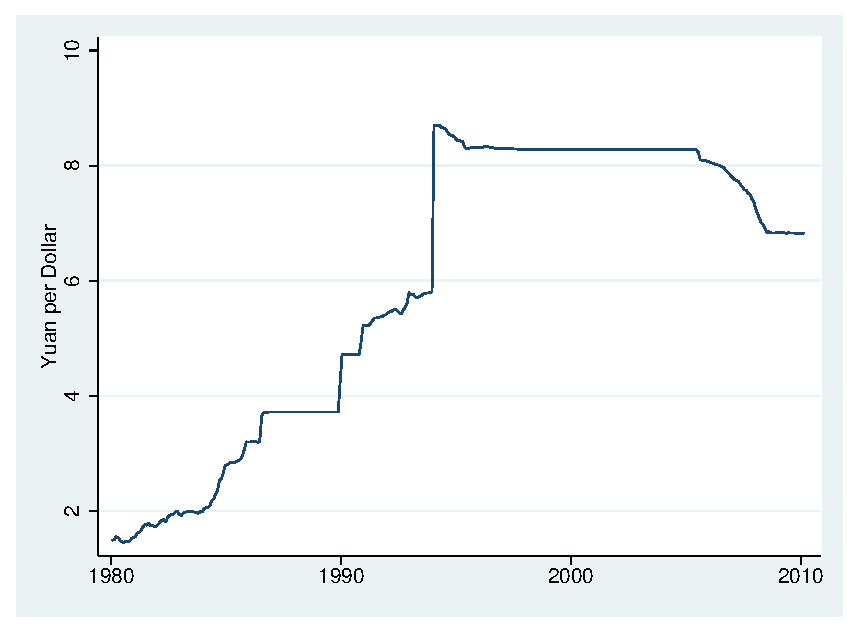
\includegraphics[width=\textwidth]{erchn.eps}

% ------------------------------------------------------
\pagebreak
\exhibit{Inflation rates in China and the US}

\bigskip%\bigskip
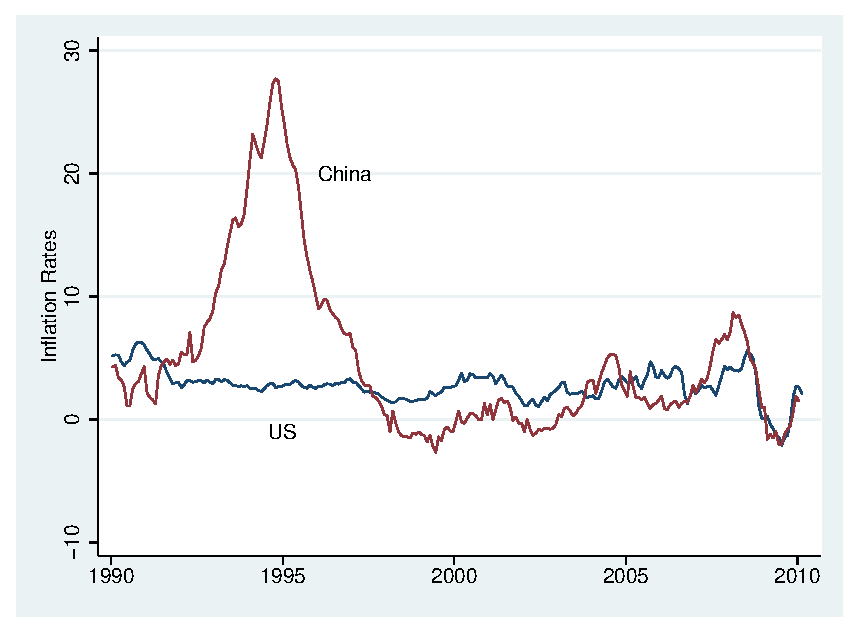
\includegraphics[width=\textwidth]{dpusachn.eps}

% ------------------------------------------------------
\pagebreak
\exhibit{The exchange rate and prices}

\bigskip%\bigskip
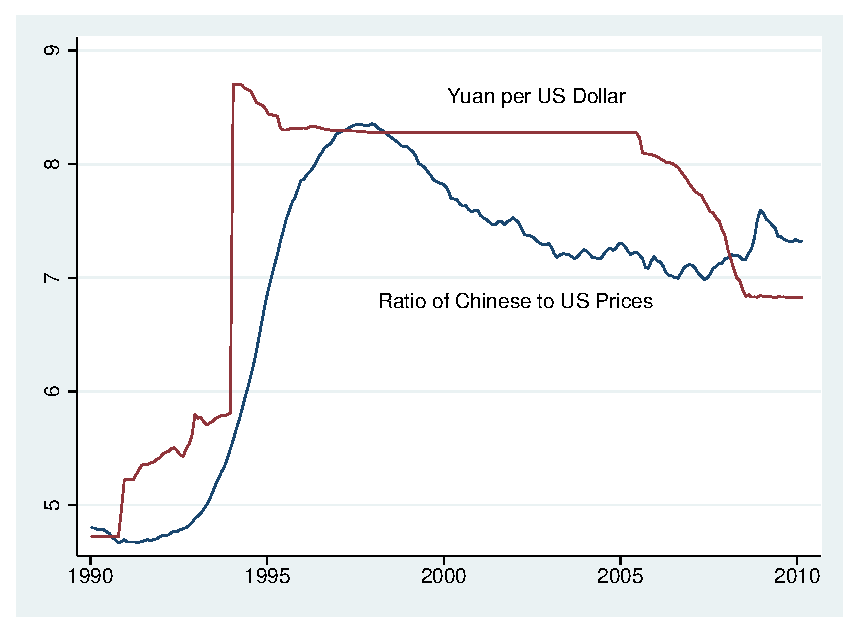
\includegraphics[width=\textwidth]{perusachn.eps}

% ------------------------------------------------------
\pagebreak
\exhibit{The real exchange rate}

\bigskip%\bigskip
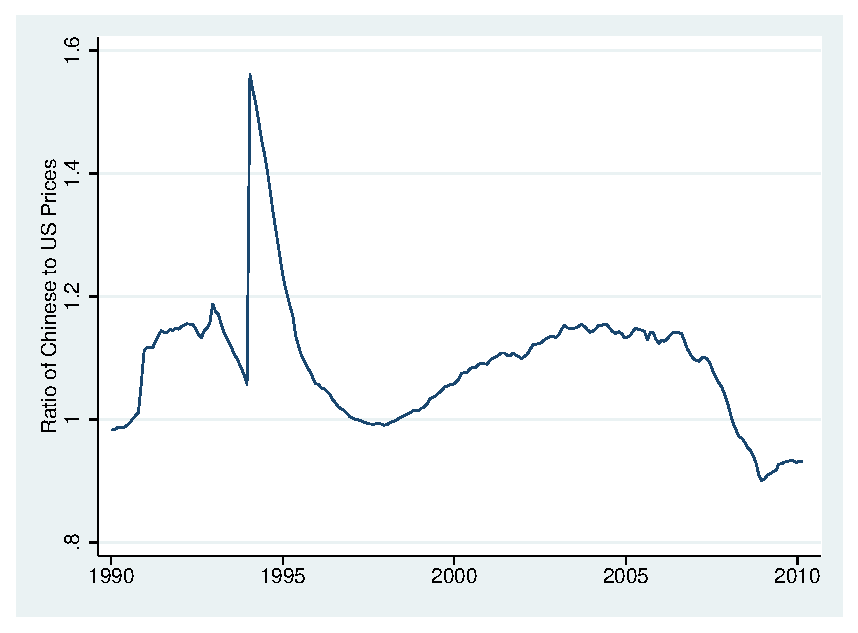
\includegraphics[width=\textwidth]{rerusachn.eps}


\vfill \centerline{\it \copyright \ \number\year 
\ NYU Stern School of Business}

\end{document} 

